\chapter{Metodologia}
\label{chap:metodologia}

Este capítulo descreve os métodos, técnicas e procedimentos que serão adotados para o desenvolvimento da proposta de solução para o Problema da Rotulação–L(2,1) utilizando algoritmos genéticos. A seguir, são apresentados os algoritmos propostos, a estrutura da base de grafos utilizada nos experimentos, os critérios de avaliação de desempenho e a metodologia de calibração de parâmetros. Também será apresentada uma abordagem baseada em \gls{pli}, utilizada como benchmark em instâncias de pequeno porte. Por fim, são descritas as etapas de experimentação e análise dos resultados. A Figura~\ref{fig:fluxo-metodologia} ilustra o fluxo metodológico geral adotado neste trabalho.

\begin{figure}[h]
    \centering
    \caption{Fluxograma da metodologia.}
    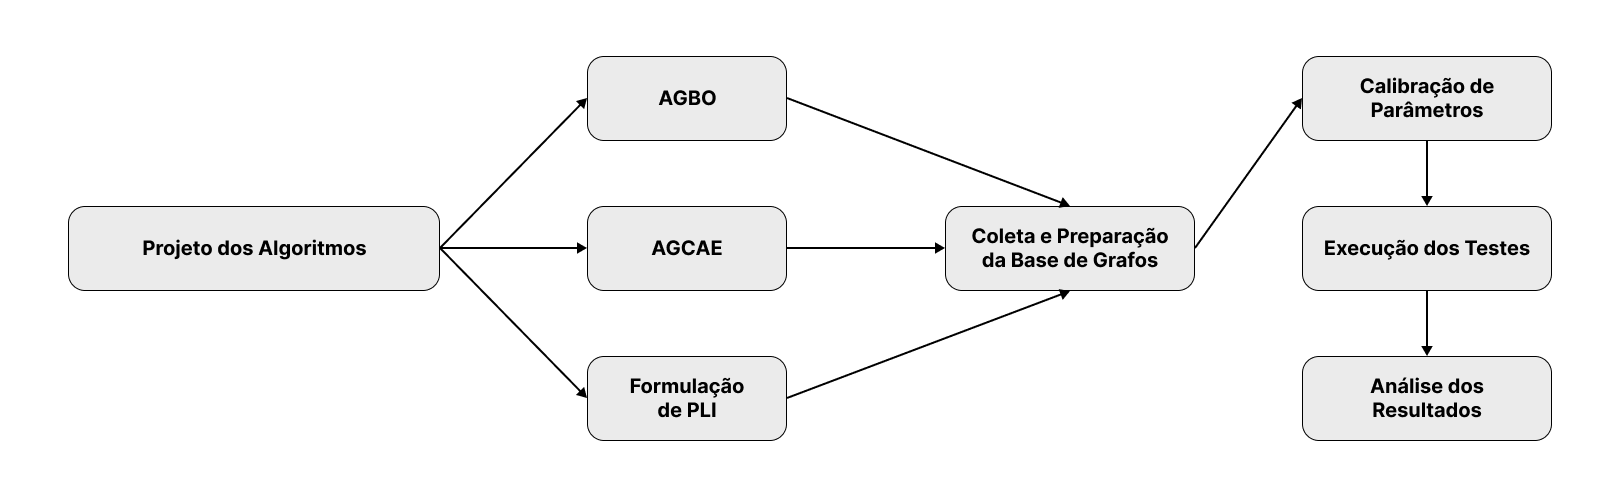
\includegraphics[width=\textwidth]{figuras/fluxo metodologia.png}
    \caption*{Fonte: Elaborado pelo autor.}
    \label{fig:fluxo-metodologia}
\end{figure}

\section{Projeto e Implementação dos Algoritmos}

Este trabalho propõe a implementação de duas abordagens evolucionárias distintas para a resolução do Problema da Rotulação–L(2,1): um \gls{agbo} e um \gls{agcae}. Além disso, será implementado um modelo baseado em \gls{pli}, conforme a formulação proposta por \citeonline{shao2013integer}, com o objetivo de fornecer soluções ótimas em instâncias de pequeno porte, servindo como referência para avaliação comparativa.

\subsection{Algoritmo Genético Baseado em Ordem}

Inspirado nas abordagens de \citeonline{coreanos}, \citeonline{indianos} e \citeonline{taranenko20042}, este algoritmo não busca construir diretamente uma rotulação. Em vez disso, o \gls{agbo} evolui uma população de permutações de vértices, e a qualidade de cada permutação é avaliada pela sua performance como entrada para uma heurística gulosa de construção da rotulação. 

Já temos uma versão preliminar desse algoritmo implementada. O algoritmo foi implementado esperando uma representação cromossômica onde cada cromossomo é representado por uma permutação dos vértices do grafo. A aptidão de um indivíduo é calculada aplicando a Heurística Gulosa descrita no Algoritmo~\ref{alg:greedy} sobre a permutação representada pelo cromossomo. Foi implementada a geração da população puramente aleatória, onde todas as soluções iniciais são permutações aleatórias dos vértices. Serão ainda implementadas, duas outras estratégias para gerar a população inicial: População Semeada com Ordem do Maior-Primeiro e População Semeada com Ordem do Menor-Último. 

Foram implementados os operadores genéticos \glsentrylong{cx} (\glsentryshort{cx}) para cruzamento e \glsentrylong{em} (\glsentryshort{em}) para mutação. Adicionalmente, serão implementados os operadores 
\glsentrylong{pmx} (\glsentryshort{pmx}), 
\glsentrylong{ox} (\glsentryshort{ox}), 
\glsentrylong{dm} (\glsentryshort{dm}), 
\glsentrylong{ivm} (\glsentryshort{ivm}), 
\glsentrylong{sm} (\glsentryshort{sm}), 
\glsentrylong{ism} (\glsentryshort{ism}) e 
\glsentrylong{sim} (\glsentryshort{sim}). Foi adotado o método de seleção por roleta viciada. Foi adotado um esquema de elitismo, que seleciona os dois indivíduos mais aptos da população. Esses indivíduos são mantidos na população da próxima geração. O critério de parada é um número fixo de gerações.

\subsection{Algoritmos Genéticos de Chaves Aleatórias Enviesadas}

Em um \gls{agcae}, cada indivíduo da população é representado por um vetor de números reais no intervalo $[0, 1]$. Assim, cada posição do vetor será associada a um vértice do grafo. A população inicial será definida por três estrategias: de forma totalmente aleatória, a ordem do maior-primeiro e do menor-último.

O decodificador ordenará os vértices com base nos valores crescentes das suas respectivas chaves. Essa ordenação define a sequência de entrada para a Heurística Gulosa (Algoritmo~\ref{alg:greedy}), que constrói uma solução viável a partir da ordem fornecida. Dessa forma, a qualidade de cada indivíduo é medida indiretamente, pela performance da heurística aplicada à sua ordenação correspondente.

\subsection{Modelo de Programação Linear Inteira}

Para estabelecer um \textit{benchmark} e obter o valor ótimo $\lambda(G)$ para instâncias de pequeno porte, será utilizado um modelo de \gls{pli}. A formulação implementada segue a proposta generalizada de \citeonline{shao2013integer}, particularizada para as restrições L(2,1). Devido à complexidade do problema, a resolução exata por meio deste modelo é computacionalmente viável apenas para grafos de tamanho reduzido. Para gerenciar o tempo de execução, será imposto um limite de tempo computacional de 1200 segundos para a execução do solver em cada instância. As soluções obtidas por esta via servirão como base para medir a qualidade e a lacuna de otimalidade das soluções encontradas pelas abordagens heurísticas. O modelo será resolvido utilizando o solver CPLEX.

\section{Coleta e Preparação da Base de Grafos}

Para garantir uma avaliação abrangente dos algoritmos propostos, será utilizada uma base experimental composta por aproximadamente 400 instâncias de grafos. Essa base contemplará as classes estruturais básicas como Árvores e Caminhos, assim como também Grafos aleatórios gerados de acordo com o modelo Erd\"{o}s-Renyi. 

Além disso, serão utilizadas instâncias de grafos provenientes das bases DIMACS e CELLAR. A coleção DIMACS foi originalmente proposta para avaliação de algoritmos de coloração e outros problemas combinatórios, sendo amplamente utilizada como \textit{benchmark} em experimentos computacionais \cite{nr, PorumbelGraphs}. Já a base CELLAR fornece instâncias de grafos estruturais e aleatórios oriundos de aplicações reais e sintéticas, e está disponível através do repositório ZIB Optimization Suite \cite{ZIB_FAP}. 

As instâncias aleatórias serão geradas por meio de ferramentas computacionais e bibliotecas como NetworkX (Python), garantindo controle sobre parâmetros como ordem e densidade. Todos os grafos serão armazenados em formato padronizado `.graphml' e validados quanto à conectividade e ausência de múltiplas arestas ou laços, conforme pressupostos do modelo de rotulação–L(2,1). Para permitir reprodutibilidade, as sementes dos geradores aleatórios utilizados na criação dos grafos serão fixadas e documentadas.

\section{Calibração de Parâmetros}

A eficácia dos algoritmos genéticos depende fortemente da escolha adequada de seus parâmetros. Dessa forma, será realizada uma fase de calibração sistemática para definir configurações apropriadas que maximizem o desempenho dos algoritmos em termos de qualidade das soluções e tempo de execução.

Como o conjunto total de instâncias é numeroso, a calibração será conduzida sobre um subconjunto representativo de grafos, selecionado de forma a cobrir diferentes tamanhos, densidades e classes estruturais. Essa seleção garantirá que os parâmetros ajustados sejam generalizáveis a um amplo espectro de instâncias.

A ferramenta \textit{irace} (\textit{Iterated Racing for Automatic Algorithm Configuration}) será empregada para automatizar o processo de ajuste dos parâmetros. Essa ferramenta utiliza uma abordagem baseada em corridas iterativas e estatísticas inferenciais para identificar, de forma eficiente, as melhores combinações de valores de parâmetros.

Os parâmetros a serem calibrados são: tamanho da população, número máximo de gerações, taxa de cruzamento ($p_c$), taxa de mutação ($p_m$), número de mutantes por geração (no caso do \gls{agcae}), parâmetro de viés $\rho$ do cruzamento no \gls{agcae} e proporção da elite (\gls{agcae}).

Cada configuração avaliada será testada em 30 execuções para contabilizar a variabilidade estocástica. As métricas consideradas durante a calibração incluirão o valor médio de $\lambda(G)$, o desvio padrão e o tempo de execução. Após a calibração, os algoritmos serão executados com as configurações mais promissoras em toda a base de grafos.

\section{Execução dos Testes e Análise dos Resultados}

Finalizada a etapa de calibração, os algoritmos serão avaliados de forma sistemática em toda a base de grafos. Cada algoritmo será executado 30 vezes para cada instância a fim de capturar a variabilidade introduzida pela natureza estocástica dos métodos evolucionários.

A análise dos resultados considerará três aspectos principais. O primeiro é o valor de $\lambda(G)$ obtido, que representa a qualidade da solução e corresponde ao maior rótulo atribuído em uma rotulação–L(2,1) válida. O segundo aspecto é o tempo de execução médio por instância, que será usado como indicador da viabilidade computacional de cada abordagem. O terceiro aspecto é a estabilidade dos algoritmos, que será avaliada pelo desvio padrão das soluções obtidas.

A comparação entre os algoritmos será feita tanto de forma quantitativa quanto estatística. Serão aplicados testes de hipóteses apropriados, como o teste de Wilcoxon pareado, para verificar a existência de diferenças significativas entre os métodos em termos de desempenho. Gráficos de dispersão entre tempo de execução e qualidade da solução auxiliarão na análise do trade-off entre precisão e custo computacional. Os resultados também serão agregados por classe de grafo.

Adicionalmente, os valores obtidos pelos algoritmos evolutivos serão comparados, sempre que possível, com os resultados exatos fornecidos pelo modelo de \gls{pli}. Essa comparação permitirá verificar a proximidade das soluções heurísticas em relação ao ótimo conhecido.

Todos os experimentos serão conduzidos em um \textit{MacBook Air} com processador \textit{Apple} M1, 8 GB de memória unificada e sistema operacional \textit{macOS}, com o uso de sementes aleatórias fixas. A implementação dos algoritmos será realizada na linguagem \textit{Python}, utilizando as bibliotecas \textit{NumPy}, \textit{NetworkX}, \textit{SciPy} e Pandas. O modelo de \gls{pli} será implementado com auxílio do pacote \textit{docplex} da IBM, que permite a formulação e resolução de modelos no solver CPLEX de forma programática em \textit{Python}. Todas as execuções serão realizadas em modo sequencial, e os tempos de execução serão cronometrados com base em medições internas de CPU. O código-fonte, as instâncias de entrada e os resultados obtidos serão devidamente documentados e disponibilizados publicamente em repositório digital, com o objetivo de garantir a reprodutibilidade e a transparência científica do estudo.

\newpage

\section{Plano de Trabalho e Cronograma}

O desenvolvimento deste trabalho foi estruturado em etapas progressivas, de modo a garantir a construção incremental dos algoritmos e a condução sistemática dos experimentos. O plano de trabalho abrange desde o levantamento bibliográfico até a redação final do relatório e preparação para a defesa. O Quadro~\ref{qua:cronograma} apresenta o cronograma de execução das etapas previstas para o desenvolvimento deste trabalho, com duração total estimada de 10 (dez) meses.

\begin{quadro}[htbp]
\centering
\caption{\label{qua:cronograma}Cronograma de execução do trabalho}
\resizebox{\textwidth}{!}{
\begin{tabular}{|p{7cm}|c|c|c|c|c|c|c|c|c|c|}
    \hline
    \textbf{Atividade} & \textbf{MAR} & \textbf{ABR} & \textbf{MAI} & \textbf{JUN} & \textbf{JUL} & \textbf{AGO} & \textbf{SET} & \textbf{OUT} & \textbf{NOV} & \textbf{DEZ} \\
    \hline
    Levantamento bibliográfico & \checkmark & & & & & & & & & \\
    \hline
    Estudo sobre rotulação–L(2,1) & \checkmark & \checkmark & \checkmark & & & & & & & \\
    \hline
    Estudo sobre algoritmos genéticos & \checkmark & \checkmark & & & & & & & & \\
    \hline
    Definição da metodologia e codificação & & & \checkmark & \checkmark & & & & & & \\
    \hline
    Implementação do \gls{agbo} & & & & \checkmark & & \checkmark & & & & \\
    \hline
    Redação do TCC I & \checkmark & \checkmark & \checkmark & \checkmark & \checkmark & & & & & \\
    \hline
    Apresentação do TCC I & & & & & \checkmark & & & & & \\
    \hline
    Revisões e ajustes & & & & & \checkmark & & & & & \\
    \hline
    Implementação do \gls{agcae} & & & & & & \checkmark & & & & \\
    \hline
    Implementação do modelo de \gls{pli} & & & & & & & \checkmark & & & \\
    \hline
    Geração e preparação da base de grafos & & & & & & & \checkmark & & & \\
    \hline
    Calibração de parâmetros com \textit{irace} & & & & & & & \checkmark & & & \\
    \hline
    Execução dos testes & & & & & & & & \checkmark & \checkmark & \\
    \hline
    Análise dos resultados & & & & & & & & \checkmark & \checkmark & \checkmark \\
    \hline
    Redação do TCC II & & & & & & & & \checkmark & \checkmark & \checkmark \\
    \hline
    Apresentação e defesa do TCC II & & & & & & & & & & \checkmark \\
    \hline
    Revisões e ajustes finais & & & & & & & & & & \checkmark \\
    \hline
\end{tabular}
}
\caption*{Fonte: Elaborado pelo autor.}
\end{quadro}